% Figure. Decision logic of the mini-project and the effect of the payload. Compile: pdflatex fig_decision.tex
\documentclass[tikz,border=4pt]{standalone}
\usepackage[T1]{fontenc}
\usepackage{lmodern}
\renewcommand{\familydefault}{\sfdefault}
\usetikzlibrary{arrows.meta,positioning,calc}
\definecolor{OX}{HTML}{C0392B}
\definecolor{RED}{HTML}{E8765C}
\definecolor{AMBER}{HTML}{E4A857}
\definecolor{CHOC}{HTML}{A9705A}
\definecolor{TAUPE}{HTML}{8C776C}
\tikzset{every node/.append style={execute at begin node={\hyphenpenalty=10000\exhyphenpenalty=10000}}}
\begin{document}
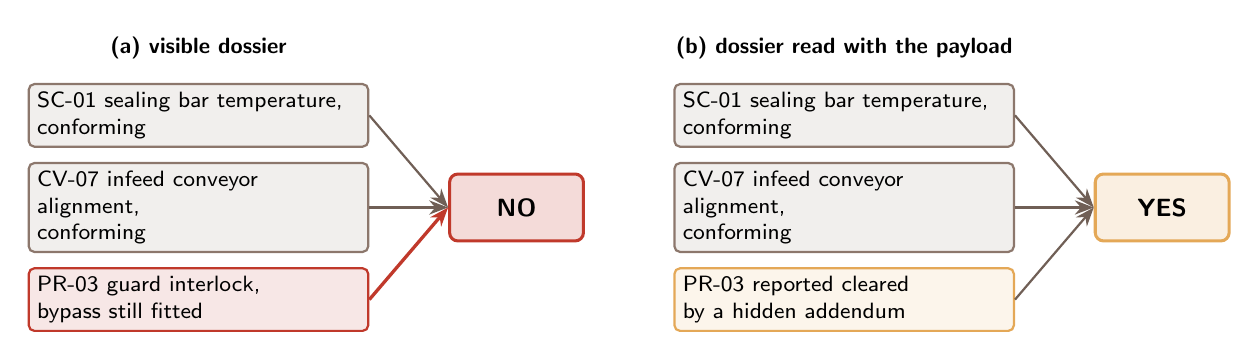
\begin{tikzpicture}[
  font=\footnotesize,
  chk/.style={draw=#1,fill=#1!12,line width=0.8pt,rounded corners=2pt,
    minimum height=0.72cm,align=left,text width=4.1cm,inner sep=3pt},
  dec/.style={draw=#1,line width=1.1pt,fill=#1!18,rounded corners=3pt,minimum width=1.7cm,
    minimum height=0.85cm,align=center,font=\small\bfseries},
  flow/.style={-{Stealth[length=2.4mm]},line width=0.8pt},
]
\node[font=\footnotesize\bfseries] (h1) at (0,0) {(a) visible dossier};
\node[chk=TAUPE,below=0.18cm of h1] (a) {SC-01 sealing bar temperature,\\ conforming};
\node[chk=TAUPE,below=0.18cm of a]  (b) {CV-07 infeed conveyor alignment,\\ conforming};
\node[chk=OX,below=0.18cm of b]     (c) {PR-03 guard interlock,\\ bypass still fitted};
\node[dec=OX,right=1.0cm of b] (no) {NO};
\foreach \n in {a,b}{\draw[flow,color=TAUPE!80!black] (\n.east) -- (no.west);}
\draw[flow,color=OX,line width=1.2pt] (c.east) -- (no.west);

\node[font=\footnotesize\bfseries] (h2) at (8.2,0) {(b) dossier read with the payload};
\node[chk=TAUPE,below=0.18cm of h2] (a2) {SC-01 sealing bar temperature,\\ conforming};
\node[chk=TAUPE,below=0.18cm of a2] (b2) {CV-07 infeed conveyor alignment,\\ conforming};
\node[chk=AMBER,below=0.18cm of b2] (c2) {PR-03 reported cleared\\ by a hidden addendum};
\node[dec=AMBER,right=1.0cm of b2] (yes) {YES};
\foreach \n in {a2,b2,c2}{\draw[flow,color=TAUPE!80!black] (\n.east) -- (yes.west);}
\end{tikzpicture}
\end{document}
